\chapter{Beyond the Standard Model}
\label{chap:BSM}

Although the \ac{SM} represents our best understanding of the elementary particles and their interactions, it does contains some deficiencies. One the one hand, it remains silent on several fronts, such as gravity, dark matter, and dark energy. One the other hand, it does not fully explain several experimental results, those in the flavor sector in particular. Two of the experimental results in the flavor sector that work against the \ac{SM} and their phenomenogical implications are discussed in \autoref{sec:BSM}. \autoref{sec:Leptoquark} introduces the leptoquark model that can be used to explain the unexpected results occurred in the flavor sector.

\section{BSM Phenomenology}
\label{sec:BSM}

As discussed in \autoref{sec:Flavor}, the renormalizable \ac{SM} Lagrangian exhibits a few continuous global symmetries, namely the $U(1)_{e}\bigotimes U(1)_{\mu}\bigotimes U(1)_{\tau}$ that give rise to the conservation of lepton family numbers. Unlike gauge symmetries of the \ac{SM}, which arise at the outset of the construction, these global $U(1)$ symmetries emerge accidentally due to the assumption (massless neutrino) that is solely driven by phenomenology. Despite the accidental nature of these symmetries, they have stood up to the tests of almost all particle physics experiments to date.  

In fact, the first and so far the only hint of the broken global symmetries didn't appear until the turn of the century through the oscillation of atmospheric neutrinos \cite{Super-Kamiokande:1998kpq,SNO:2002tuh}. This remarkable observation directed significant interest from both theorists and experimentalists to the flavor sector of the \ac{SM}. On the one hand, it cements the calls for extensions of the \ac{SM} by demonstrating the mixing of neutrino flavors. On the other hand, it also suggests that the $U(1)$ symmetries are indeed broken, and the \ac{CLFV} should also occur. 

\begin{figure}[tbh!]
 \begin{center}
 \begin{tabular}{c}
 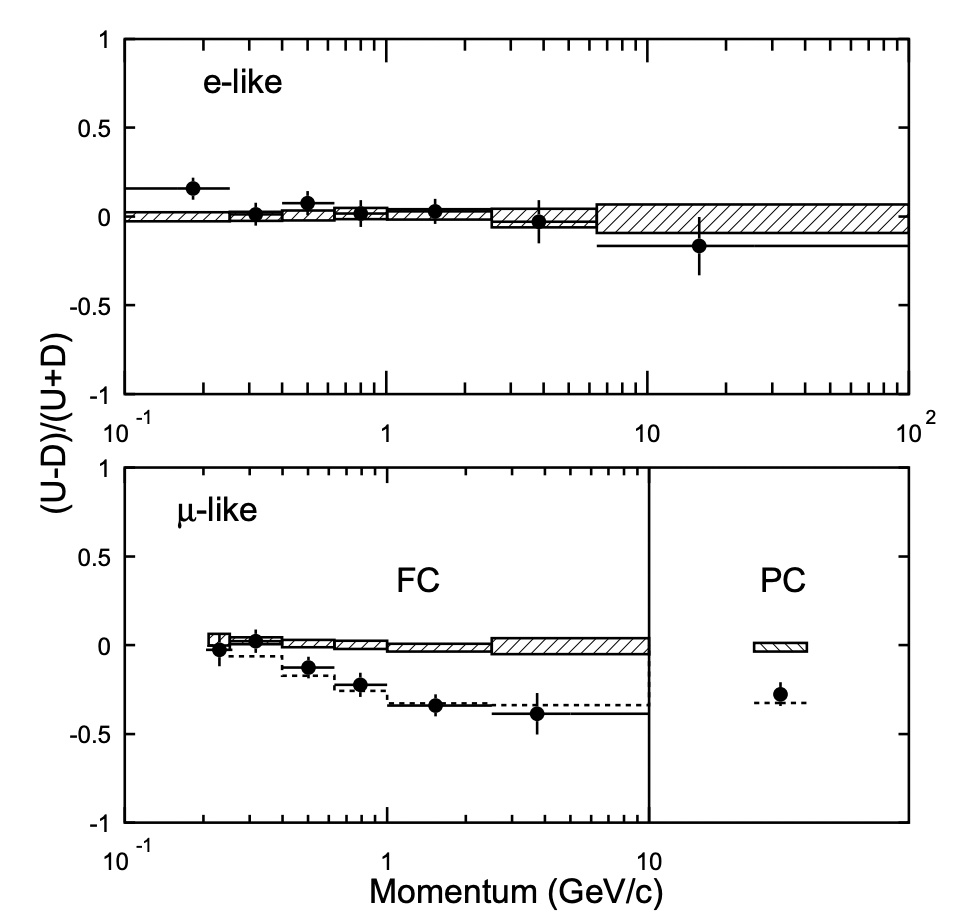
\includegraphics[width=0.55\textwidth]{figures/Part1/BSM/SuperK}
 \end{tabular}
 \caption{Cloud chamber photograph taken from Anderson's 1932 paper~\cite{Super-Kamiokande:1998kpq}. The upper chamber and the lower chamber is separated by a 6 mm lead plate. The deflection and direction of the particle's ion trail indicate that the particle is a positron.}
 \label{fig:Positron}
 \end{center}
\end{figure}

Although the exact mechanism behind neutrino mass remains unclear, it can be induced through two distinct ways that only require minimal departures from the original formulation of the \ac{SM}. By adding right-handed neutrino fields, the Yukawa coupling \cite{Weinberg:1967tq} that describes the emergence of Dirac fermion masses can be naturally extended to neutrinos. The neutrino mass can also be realized by introducing the nonrenormalizable Dimension-5 operator \cite{Weinberg:1979sa}, known as the Weinberg operator. This operator gives rise to Majorana neutrino mass terms upon spontaneous symmetry breaking. 

In either case, the masses of neutrinos are accounted for and the strength of the neutrino flavor mixing is governed by the \ac{PMNS} matrix \cite{Pontecorvo:1957cp,Maki:1962mu}, a nearly perfect analog to the \ac{CKM} matrix \cite{Cabibbo:1963yz,Kobayashi:1973fv} that describes quark mixing in the weak interaction. The same \ac{PMNS} matrix can also give rise to the \ac{CLFV} process through loop diagrams involving charged current. However, these diagrams are highly suppressed and phenomenologically negligible due to the small neutrino mass relative to the electroweak scale. Therefore, any experimental observation of \ac{CLFV} will be unambiguous evidence of new physics beyond the \ac{SM}.

Recent flavor anomalies reported by the \ac{LHCb} experiment~\cite{LHCb:2023zxo} mark the first major deviation from the SM produced by the \ac{LHC}. Not only did this result provide a direct hint towards \ac{LFUV}, it also prompted renewed experimental interest in \ac{CLFV} search since models that accommodate \ac{LFUV} generally give rise to \ac{CLFV} as well ~cite{Glashow:2014iga}. The \ac{LHC} provides the best sensitivity to \ac{CLFV} processes involving a heavy leg, such as a top quark or a Higgs boson. Moreover, some of these models~\cite{Kim:2018oih} also suggest that \ac{CLFV} involving a top quark is within the reach of the \ac{LHC} sensitivity. Therefore, a search for \ac{CLFV} in the top quark sector could shed light on these flavor anomalies and further our understanding of the broken global symmetries.

\begin{figure}[tbh!]
 \begin{center}
 \begin{tabular}{c}
 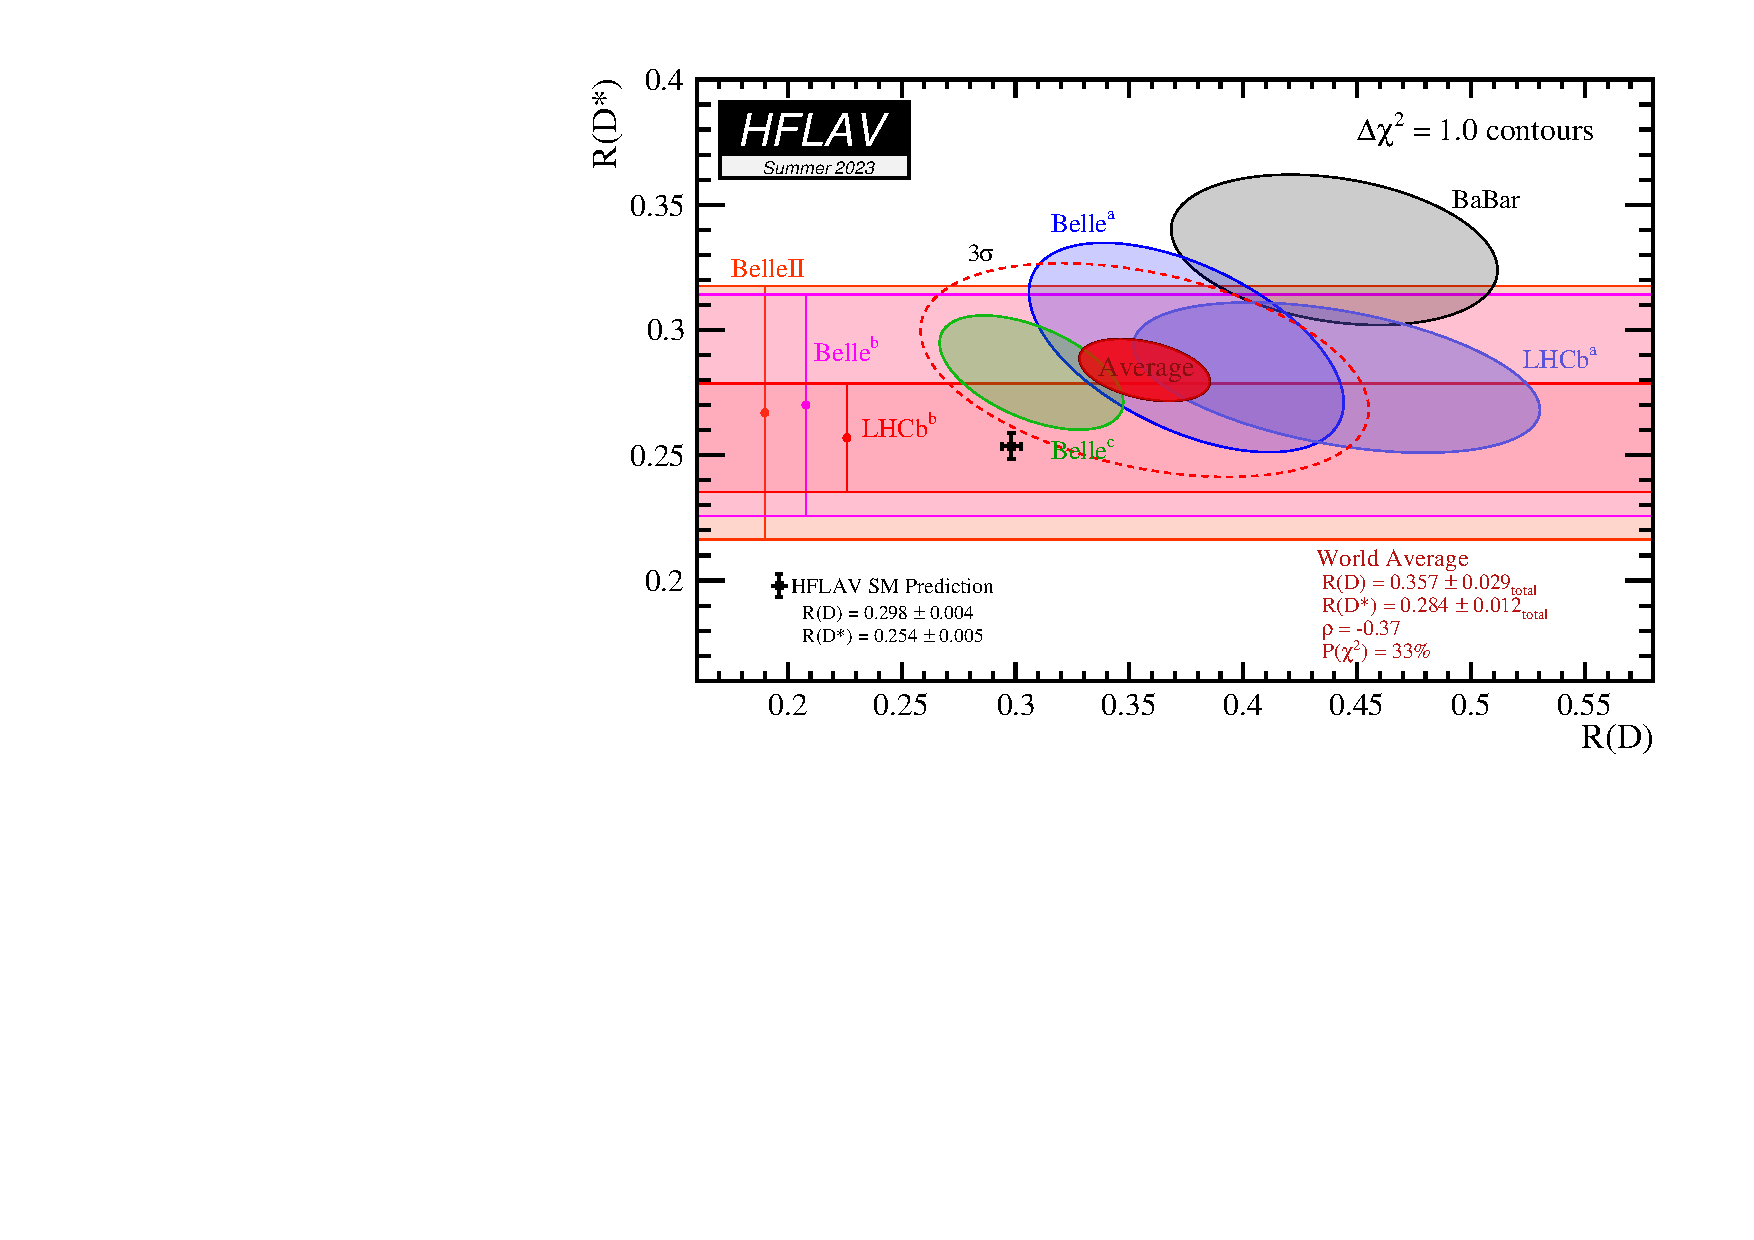
\includegraphics[width=0.6\textwidth]{figures/Part1/BSM/RD}
 \end{tabular}
 \caption{Cloud chamber photograph taken from Anderson's 1932 paper~\cite{HFLAV}. The upper chamber and the lower chamber is separated by a 6 mm lead plate. The deflection and direction of the particle's ion trail indicate that the particle is a positron.}
 \label{fig:Positron}
 \end{center}
\end{figure}

\section{Leptoquark Model}
\label{sec:Leptoquark}

\cite{Pati:1973uk}